\chapter{Introducción} 
\label{ch:introduccion}
Desde hace décadas, sobre todo con el Big data, la cantidad de información que se mueve por internet y que deben controlan las empresas ha aumentado mucho. \\ Toda la distribución, almacenamiento y procesado de la información se ha ido descentralizando, y ha dejado de hacerse en las propias oficinas para realizarse en unas salas especializadas llamadas \textit{Centros de Procesamiento de Datos} o \textit{CPD}. \\ Estas salas están llenas de equipamiento informático funcionando de manera continua bajo unas condiciones óptimas para su correcto funcionamiento y mantenimiento, por lo que además están equipadas con multitud de sistemas de control para evitar cualquier tipo de incidente, que supusiera perdida de información o de servicio.

Este trabajo está dirigido al diseño e implementación de uno de esos sistemas de control que poseen los CPD, pero primero en este capítulo se presentaran las motivaciones para su desarrollo y objetivos de este. También se presentará la metodología de trabajo y como se estructura el proyecto.

\section{Motivación del trabajo}
MEDIA CARA - CARA

\section{Objetivos}
El objetivo de este proyecto es desarrollar un dispositivo capaz de captar y almacenar varias medidas ambientales del CPD, junto a video en tiempo real del lugar. \\ El dispositivo pretende ser de bajo presupuesto, capaz de detectar riesgos y proporcionar una visión general del ambiente de la sala, pero no contará con la precisión de equipos de altas capacidades. Su bajo coste posibilitará que se pueda usar en entornos de menor escala o con presupuestos ajustados.  \\ Como se ha dicho los datos se almacenarán en una base de datos, que también será creada y gestionada correspondientemente para poder consultarlos en cualquier momento y analizarlos en busca de cualquier problema o mejora del sistema. \\ Además se desarrollará una página web que permitirá acceder a la información obtenida por estos dispositivos vía web, para poder ser consultada desde cualquier dispositivo con acceso a internet. \\ Otros objetivos relacionados son:
\begin{itemize}
    \item Acceso a la información de los diferentes dispositivos de medida conectados, para gestionar los diferentes dispositivos de manera más sencilla.
    \item Base de datos y servidor web siempre accesible en la red, para no perderse los posibles incidentes en ningún momento.
    \item Sistema de seguridad mediante inicio de sesión para acceder a los datos e imagen tomada.
    \item Página web simple e intuitiva, para facilitar la gestión de la información mostrada.
    \item Página web responsive para móvil, tablet y ordenador.
\end{itemize}

\section{Metodología}
La metodología que se emplea en este proyecto es Métrica V3 \cite{portal_administracion_electronica_metrica_nodate} con algunas pequeñas modificaciones para que se adapte mejor al trabajo que vamos a desarrollar. \\ Lo bueno de emplear una metodología es que nos permite seguir el ciclo de vida del proyecto en un orden adecuado. además, uno de sus aspectos más importantes es que su capacidad para adaptarse a esta clase de proyectos, y también que tiene presente durante todo el proceso las necesidades del cliente, en forma de requisitos. \\ Se muestra a continuación un diagrama de Métrica V3 elaborado por el Ministerio de Administraciones Públicas para que se pueda entender como es este ciclo:

\begin{figure}[H]
	\ffigbox[\FBwidth]
	{\caption[Diagrama Métrica V3]{Diagrama Métrica V3 \cite{portal_administracion_electronica_metrica_nodate}}}
	{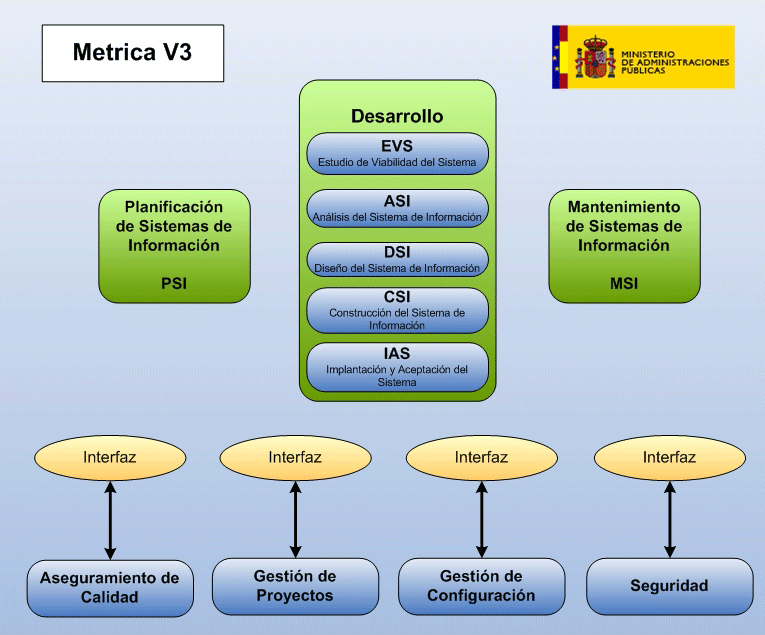
\includegraphics[scale=0.6]{Metrica3.png}}
\end{figure}

\section{Estructura del documento}
En esta sección se presentan los diferentes capítulos que conforman este documento, para que se pueda entender mejor las diferentes fases de Métrica V3 aplicadas que completan el ciclo de desarrollo del proyecto. \\ Capítulos en los que se divide el documento:

\begin{itemize}
    \item \textbf{Introducción:} Este capítulo tiene como propósito presentar al lector el tema que se tratara antes de profundizar en él durante todo el documento. También se presentan las motivaciones que se han tenido para la elección de este tema y los objetivos de este. Por último, explica la estructura y metodología que sigue el contenido. 
    \item \textbf{Estado del arte:} Consiste en un análisis de la situación actual del producto que planeamos desarrollar, buscando soluciones existentes que hagan lo mismo o algo parecido. Después de conocer esas soluciones se buscan los puntos fuertes de cada una de ellas, en busca de un hueco que podamos cubrir con nuestro producto.
    \item \textbf{Análisis del sistema (ASI):}
    \item \textbf{Diseño del sistema (DSI):}
    \item \textbf{Implementación (CSI):}
    \item \textbf{Pruebas:}
    \item \textbf{Gestión del proyecto (PSI):} Expone la planificación temporal que se ha llevado del proyecto, indicando los tiempos que han llevado cada una de las partes del documento, acompañado de un diagrama de Gantt. \\ Este capítulo también comprende el presupuesto, en el que se presentan de manera desglosada todos los gastos asociados al proyecto y finaliza con un resumen en el que se indica el precio de proyecto para un cliente.
    \item \textbf{Marco regulador:} Recoge los aspectos legales relacionados con el proyecto, con las tecnologías que se han empleado y el impacto de nuestro sistema.
    \item \textbf{Conclusiones:} Es el último capítulo que se escribe, en el que se recoge tras todo el proceso de diseño e implementación cuáles han sido las impresiones finales del proyecto y a modo personal. \\ Esta concluye con una mirada al futuro, con posibles aplicaciones que se le podrán dar y analizando cuáles serían posibles mejoras y funcionalidades para el producto. 
    \item \textbf{Bibliografía:} Recoge las referencias a todos los recursos que han sido consultados durante la realización de este documento, con el propósito de dar validez a la información que se ha presentado y si fuera necesario profundizar más en algún punto.
\end{itemize}